\documentclass[11pt, oneside]{article}
\usepackage{geometry}
\geometry{letterpaper}
\usepackage{graphicx}
\usepackage{amssymb}
\usepackage{amsmath}
\usepackage{tikz}
\usepackage{tikz-qtree}

\title{SICP Exercise 2.24}
\author{Yuchong Pan}

\begin{document}
\maketitle

\begin{center}
    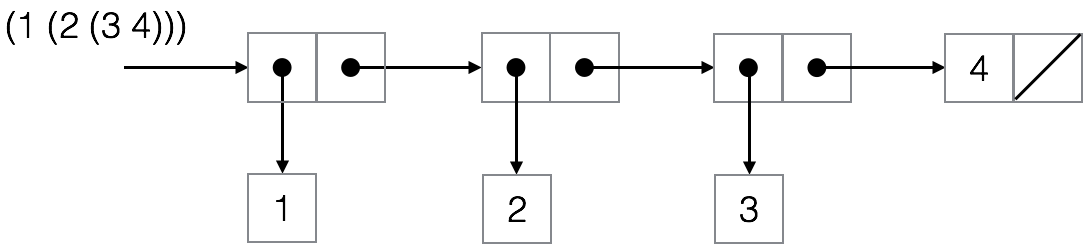
\includegraphics[height=3cm]{box-and-pointer.png}
    
    ~

    ~

    ~

    \begin{tikzpicture}
        \node (isroot) {(1 (2 (3 4)))}
            [sibling distance=7cm]
            child { node {1} }
            child {
                node {(2 (3 4))}
                    [sibling distance=7cm]
                    child { node {2} }
                    child {
                        node {(3 4)}
                            [sibling distance=7cm]
                            child{ node {3} }
                            child{ node {4} }
                    }
            };
    \end{tikzpicture}
\end{center}

\end{document}
